\documentclass[UTF8,11pt,a4paper,fontset=fandol]{ctexart}
\usepackage[margin=2.35cm,headheight=15pt]{geometry}
\usepackage{amsmath,amssymb,bm,booktabs,array,graphicx,float,enumitem}
\usepackage{fontspec,xcolor,fancyhdr,caption,placeins,hyperref}
\setmainfont{texgyretermes-regular.otf}[BoldFont=texgyretermes-bold.otf,
 ItalicFont=texgyretermes-italic.otf,BoldItalicFont=texgyretermes-bolditalic.otf]
\setsansfont{texgyreheros-regular.otf}[BoldFont=texgyreheros-bold.otf]
\setmonofont{lmmono10-regular.otf}
\definecolor{ink}{HTML}{235789}
\hypersetup{colorlinks=true,linkcolor=ink,urlcolor=ink,citecolor=ink,
 pdftitle={基于近端梯度法的 Lasso 稀疏回归求解与数值实验},
 pdfauthor={毛语菲（学号：10255102560）}}
\ctexset{section={format=\Large\bfseries\color{ink}},subsection={format=\large\bfseries}}
\pagestyle{fancy}
\fancyhf{}
\fancyhead[L]{\small 最优化方法研究报告}
\fancyhead[R]{\small Lasso 与近端梯度法}
\fancyfoot[C]{\thepage}
\renewcommand{\headrulewidth}{0.3pt}
\captionsetup{font=small,labelfont=bf,labelsep=quad}
\setlist{nosep,leftmargin=2em}
\setlength{\parskip}{0.22em}
\linespread{1.18}
\setlength{\emergencystretch}{2em}
\renewcommand{\topfraction}{0.92}
\renewcommand{\bottomfraction}{0.85}
\renewcommand{\textfraction}{0.06}
\renewcommand{\floatpagefraction}{0.8}
\setcounter{topnumber}{4}
\setcounter{bottomnumber}{3}
\setcounter{totalnumber}{6}
\newcommand{\R}{\mathbb{R}}
\newcommand{\soft}{\mathcal{S}}
\newcommand{\norm}[1]{\left\|#1\right\|}
% Generated from actual results; do not hand-edit.
\newcommand{\IterSpeedIndependent}{1.10}
\newcommand{\TimeSpeedIndependent}{1.07}
\newcommand{\IterSpeedCorrelated}{1.44}
\newcommand{\TimeSpeedCorrelated}{1.39}
\newcommand{\BaseMSE}{$0.348\pm0.057$}
\newcommand{\BaseError}{$0.0738\pm0.0124$}
\newcommand{\BaseErrorMean}{0.0738}
\newcommand{\BaseNNZ}{77.0}
\newcommand{\BasePrecision}{0.274}
\newcommand{\BaseRecall}{1.000}
\newcommand{\BaseNoiseVariance}{0.2208}
\newcommand{\BaseNoiseRatio}{1.57}
\newcommand{\CPUName}{Apple M4}
\newcommand{\PythonVersion}{3.13.12}
\newcommand{\NumpyVersion}{2.2.6}
\newcommand{\ScipyVersion}{1.15.3}
\newcommand{\SpectralMilliseconds}{5.04}
\newcommand{\MaxObjectiveDifference}{$3.90\times10^{-12}$}
\newcommand{\MaxReferenceResidual}{$2.29\times10^{-11}$}
\newcommand{\SmallStepIterations}{1240.8}
\newcommand{\FullStepIterations}{305.6}
\newcommand{\TotalSeconds}{72.5}
\newcommand{\ExampleNNZ}{63}
\newcommand{\ExampleTP}{20}
\newcommand{\ExampleFP}{43}
\newcommand{\ErrorLowSample}{0.1291}
\newcommand{\ErrorHighSample}{0.0509}
\newcommand{\MSELowSample}{0.6023}
\newcommand{\MSEHighSample}{0.2782}
\newcommand{\ErrorLowNoise}{0.0368}
\newcommand{\ErrorHighNoise}{0.2293}
\newcommand{\ErrorHighCorrelation}{0.1257}


\title{\vspace{-1.5em}\textbf{基于近端梯度法的 Lasso\\稀疏回归求解与数值实验}}
\author{毛语菲（学号：10255102560）}
\date{2026 年 10 月 31 日}

\begin{document}
\maketitle
\thispagestyle{fancy}
\begin{abstract}
针对高维线性回归中参数数目超过样本数、且真实参数具有稀疏性的情形，本文研究
带 $\ell_1$ 正则化的 Lasso 模型。通过分离光滑损失项与非光滑正则项，推导软阈值近端算子，
独立实现近端梯度法 ISTA，并以标准 FISTA 作为加速对照。采用 $p=1000$、真实稀疏度 $s=20$
的高斯随机回归问题，在 5 个固定随机种子下开展算法收敛、步长、正则化强度及数据难度实验。
两种方法均以归一化 KKT 残差和原始--对偶间隙同时不超过 $10^{-6}$ 为停止条件，
并与高精度坐标下降结果交叉验证。
在独立特征和相关系数 $\rho=0.8$ 的算法基准中，FISTA 相对 ISTA 的平均迭代数比值
分别对应约 \IterSpeedIndependent{} 倍和 \IterSpeedCorrelated{} 倍的加速。
基础场景经验证集选参后，测试均方误差为 \BaseMSE{}，参数相对误差为 \BaseError{}；
平均选择 \BaseNNZ{} 个变量，说明预测效果与精确支持集恢复并不等价。
全部报告数值来自配套程序的实际运行，提供原始 CSV、迭代轨迹、图表和复现脚本。
\end{abstract}
\noindent\textbf{关键词：}Lasso；近端梯度法；ISTA；FISTA；稀疏回归；数值优化
\par\noindent\textbf{代码与数据：}\url{https://github.com/10255102560/Lasson}

\section{研究背景与研究问题}
在传感器测量、信号重建或包含大量候选因素的回归建模中，常会遇到变量数多于观测数的情况。
若仅最小化训练残差，可能存在多个拟合良好的参数向量；训练误差很小也不代表对新数据预测准确。
当先验认为只有少数变量真正起作用时，可以在拟合误差之外增加稀疏性约束。
Lasso 通过对参数的绝对值之和施加惩罚，同时完成回归和变量筛选\cite{tibshirani}。

本文采用任务允许的\textbf{随机生成问题}，而非声称使用某个真实业务数据集。
这样可以同时知道真实参数和噪声水平，在可控条件下检验算法与模型。
研究围绕三个问题展开：第一，如何将 Lasso 的非光滑优化转化为易于实现的迭代；
第二，ISTA 与 FISTA 在相同精度下的计算表现如何；第三，步长、正则化强度、样本量、噪声和相关性如何影响结果。
这里区分\textbf{优化误差}与\textbf{统计误差}：前者衡量离 Lasso 最优值还有多远，后者衡量估计参数或预测结果离真实机制有多远。

\section{数学模型与最优性条件}
\subsection{Lasso 模型}
设 $A\in\R^{n\times p}$ 为经过训练集标准化的特征矩阵，$b\in\R^n$ 为中心化后的响应，研究
\begin{equation}
 \min_{x\in\R^p} F(x)=f(x)+g(x)
 =\frac{1}{2n}\norm{Ax-b}_2^2+\lambda\norm{x}_1,\qquad \lambda>0.
 \label{eq:lasso}
\end{equation}
其中 $f$ 衡量拟合误差，$g$ 鼓励稀疏。$F$ 是连续凸函数，且 $\lambda\norm{x}_1$ 保证其水平集有界，因此存在最优解。
由于 $p>n$ 时 $A^\top A$ 不满秩，不能仅凭这一模型宣称全局强凸、参数解必然唯一或全局线性收敛。
本文比较目标值和最优性证书，不将求解器参数完全相等作为一般性的正确性要求。

光滑部分满足
\begin{equation}
 \nabla f(x)=\frac{1}{n}A^\top(Ax-b),\qquad
 \nabla^2 f(x)=\frac{1}{n}A^\top A,\qquad
 L=\frac{\norm{A}_2^2}{n}.
 \label{eq:gradient}
\end{equation}
$L$ 是梯度的 Lipschitz 常数。这里矩阵 $2$ 范数为最大奇异值，\textbf{不是 Frobenius 范数}。

\subsection{KKT 条件与零解阈值}
令 $q=\nabla f(x)$。由凸问题的一阶最优性条件，$x$ 最优当且仅当
\begin{equation}
 0\in q+\lambda\partial\norm{x}_1,
 \quad\text{即}\quad
 \begin{cases}
 q_j+\lambda\operatorname{sign}(x_j)=0,&x_j\ne0,\\
 |q_j|\le\lambda,&x_j=0.
 \end{cases}
 \label{eq:kkt}
\end{equation}
代入 $x=0$，可知当 $\lambda\ge\lambda_{\max}$ 时，零向量是一个最优解，其中
\begin{equation}
 \lambda_{\max}=\frac{\norm{A^\top b}_\infty}{n}.
 \label{eq:lambdamax}
\end{equation}
因此用 $\lambda/\lambda_{\max}$ 描述正则化强度，比直接给出一组与数据尺度无关的绝对数值更清楚。

\section{近端梯度法的推导与实现}
\subsection{从二次上界到近端更新}
因为 $\ell_1$ 范数在零点不可微，普通光滑梯度下降公式不能直接用于整个 $F$。
在当前点 $x^k$ 线性化 $f$，并加入二次稳定项，得到
\begin{equation}
 x^{k+1}=\mathop{\arg\min}_{z}\left\{
 f(x^k)+\langle\nabla f(x^k),z-x^k\rangle
 +\frac{1}{2\eta}\norm{z-x^k}_2^2+g(z)\right\}.
 \label{eq:surrogate}
\end{equation}
配方并去掉与 $z$ 无关的项，记 $v=x^k-\eta\nabla f(x^k)$，则
\begin{equation}
 x^{k+1}=\operatorname{prox}_{\eta g}(v)
 =\mathop{\arg\min}_{z}\left\{\frac12\norm{z-v}_2^2+\eta\lambda\norm{z}_1\right\}.
\end{equation}
该问题按坐标分离。对标量问题 $\min_u\frac12(u-v_j)^2+\tau|u|$，
分别考察 $u>0$、$u<0$、$u=0$：前两种情形的一阶条件给出 $u=v_j-\tau$ 和 $u=v_j+\tau$；
第三种情形要求 $v_j\in[-\tau,\tau]$。于是得到软阈值算子
\begin{equation}
 \soft_\tau(v_j)=\begin{cases}
 v_j-\tau,&v_j>\tau,\\
 0,&|v_j|\le\tau,\\
 v_j+\tau,&v_j<-\tau,
 \end{cases}
 =\operatorname{sign}(v_j)\max\{|v_j|-\tau,0\}.
\end{equation}
最终，Lasso 的近端梯度迭代为
\begin{equation}
 \boxed{x^{k+1}=\soft_{\eta\lambda}\!\left(x^k-\frac{\eta}{n}A^\top(Ax^k-b)\right).}
 \label{eq:ista}
\end{equation}
阈值必须是 $\eta\lambda$，且梯度中的 $1/n$ 必须与目标函数的定义保持一致。
每次更新将较小分量置零，并将较大分量向零收缩，这同时解释了稀疏性和参数收缩偏差。
迭代阈值方法在稀疏逆问题中的研究可参见文献\cite{daubechies}。

\subsection{步长、下降性质与收敛率}
取 $0<\eta\le1/L$ 时，式\eqref{eq:surrogate}中的函数是 $F$ 的上界，且在 $x^k$ 处取等号。
记此上界为 $Q_\eta(z;x^k)$，则
\begin{equation}
 F(x^{k+1})\le Q_\eta(x^{k+1};x^k)
 \le Q_\eta(x^k;x^k)=F(x^k).
\end{equation}
因此 ISTA 的目标函数值单调不增。对任意最优解 $x^\star$，近端最优性还给出
\begin{equation}
 F(x^{k+1})-F(x^\star)
 \le\frac{\norm{x^k-x^\star}_2^2-\norm{x^{k+1}-x^\star}_2^2}{2\eta}.
\end{equation}
将其求和，并结合目标值的单调性，可得
\begin{equation}
 F(x^k)-F(x^\star)\le\frac{\norm{x^0-x^\star}_2^2}{2\eta k}.
 \label{eq:istarate}
\end{equation}
特别地，$\eta=1/L$ 时为 $O(1/k)$ 的最坏情形目标误差界\cite{beck}。
这一上界不意味着每个实例的实测曲线都严格按 $1/k$ 衰减，也不直接给出参数恢复误差的速率。

\subsection{FISTA 加速对照}
为考察动量的影响，加入未使用重启策略的标准 FISTA。设 $x^0=y^0=0$、$t_0=1$，依次计算
\begin{align}
 x^{k+1}&=\soft_{\lambda/L}\left(y^k-\frac{1}{L}\nabla f(y^k)\right),\\
 t_{k+1}&=\frac{1+\sqrt{1+4t_k^2}}{2},\\
 y^{k+1}&=x^{k+1}+\frac{t_k-1}{t_{k+1}}(x^{k+1}-x^k).
\end{align}
在同样的凸性和 Lipschitz 梯度条件下，FISTA 满足\cite{beck}
\begin{equation}
 F(x^k)-F(x^\star)\le
 \frac{2L\norm{x^0-x^\star}_2^2}{(k+1)^2}.
 \label{eq:fistarate}
\end{equation}
其目标值不保证逐步单调。理论比较针对目标误差的最坏情形上界，并不保证在每个实例、
每个精度或以 KKT 残差作为停止条件时，FISTA 都比 ISTA 快。

对本研究的二次损失，梯度是仿射函数，故对任意动量系数 $a$ 有
\begin{equation}
 \nabla f\big(x^k+a(x^k-x^{k-1})\big)
 =\nabla f(x^k)+a\big(\nabla f(x^k)-\nabla f(x^{k-1})\big).
\end{equation}
实现据此复用梯度，使两种方法每轮均只需一次 $A$ 和一次 $A^\top$ 的矩阵--向量乘法，
同时得到新点的最优性证书。密集矩阵下每轮代价为 $O(np)$，除矩阵外的工作存储为 $O(n+p)$。

\subsection{停止条件与数值证书}
仅观察目标函数变化小可能过早停止。本文同时要求\textbf{归一化 KKT 残差}和\textbf{归一化原始--对偶间隙}
均不大于 $10^{-6}$。定义
\begin{equation}
 v_j(x)=\begin{cases}|q_j+\lambda\operatorname{sign}(x_j)|,&x_j\ne0,\\
 (|q_j|-\lambda)_+,&x_j=0,
 \end{cases}
 \qquad R_{\rm KKT}(x)=\frac{\norm{v(x)}_\infty}{\max\{1,\lambda_{\max}\}}.
\end{equation}
KKT 计算使用算法给出的精确零分量；统计支持集时另用 $10^{-5}$ 阈值，两者用途不同。

为得到可计算的目标误差上界，令 $e=b-Ax$，由约束表示
$e=b-Ax$ 的拉格朗日函数消去 $e,x$，可得对偶问题
\begin{equation}
 \max_\theta D(\theta)=b^\top\theta-\frac n2\norm{\theta}_2^2,
 \qquad \norm{A^\top\theta}_\infty\le\lambda.
\end{equation}
用残差构造可行点
\begin{equation}
 \theta=\frac{e}{n c},\qquad
 c=\max\left\{1,\frac{\norm{A^\top e}_\infty}{n\lambda}\right\}.
\end{equation}
由弱对偶性，$0\le F(x)-F(x^\star)\le F(x)-D(\theta)$。
因此使用
\begin{equation}
 G_{\rm rel}(x)=\frac{F(x)-D(\theta)}{\max\{1,|F(x)|\}},\qquad
 \max\{R_{\rm KKT}(x),G_{\rm rel}(x)\}\le10^{-6}
 \label{eq:stop}
\end{equation}
作为共同停止准则。程序只把浮点舍入量级的负间隙截为零，显著负值会触发错误。
另设 50000 次迭代上限；未达到准则的结果不会被标记为收敛。

\section{实验设计与可复现设置}
\subsection{数据生成、预处理与划分}
在原始坐标下生成
\begin{equation}
 Z_{i,:}\sim\mathcal{N}(0,\Sigma),\qquad
 \Sigma_{jk}=\rho^{|j-k|},\qquad
 y=Z\beta_{\rm true}+\varepsilon,\quad
 \varepsilon\sim\mathcal{N}(0,\sigma^2I).
\end{equation}
从 $p=1000$ 个坐标中均匀无放回选取 $s=20$ 个，非零系数的符号等概率取正负，
绝对值服从 $\operatorname{Uniform}(0.5,1.5)$。设
\begin{equation}
 \sigma=\delta\sqrt{\beta_{\rm true}^\top\Sigma\beta_{\rm true}},
 \qquad \operatorname{SNR}_{\rm dB}=-20\log_{10}\delta.
\end{equation}
基础场景取 $n=300$、$\rho=0$、$\delta=0.1$，即总体信噪比为 20 dB。
验证集和测试集分别有 300、1000 个独立样本。三组数据共享真实参数，使用独立随机子流。

仅由训练集计算每列均值 $\mu_j$、标准差 $s_j$（分母为 $n$）和响应均值 $\bar y$，
令 $A_{ij}=(Z_{ij}-\mu_j)/s_j$、$b_i=y_i-\bar y$。
验证集和测试集均沿用这些训练统计量。
求得 $\hat x$ 后，原始尺度参数为 $\hat\beta_j=\hat x_j/s_j$，预测值为
\begin{equation}
 \hat y(z)=(z-\mu)^\top\hat\beta+\bar y.
\end{equation}
因此截距没有受到 $\ell_1$ 惩罚，也没有用验证或测试数据重新估计标准化参数。

固定随机种子为 20261031、20261101、20261102、20261103、20261104。
同一随机种子在各难度条件下复用真实参数和对应随机子流，以减少无关随机差异。
表中的“均值 $\pm$ 标准差”均为这 5 次独立种子实验的样本标准差（分母为 4），并非置信区间。

\subsection{实验分组与参数选择}
\begin{table}[htbp]
\centering\small
\caption{实验设置；未说明的参数均取基础场景数值}
\begin{tabular}{p{2.5cm}p{10.4cm}}
\toprule
实验 & 设置及目的\\
\midrule
算法比较 & $\rho\in\{0,0.8\}$，固定 $\lambda=0.05\lambda_{\max}$；两算法从零初始化、同精度停止。\\
步长实验 & ISTA 使用 $\eta\in\{0.25/L,0.5/L,1/L\}$，固定 $\lambda=0.05\lambda_{\max}$。\\
正则化实验 & $\lambda/\lambda_{\max}\in\{0.001,0.003,0.01,0.03,0.1,0.3,1\}$；每个候选均从零初始化。\\
样本量实验 & $n\in\{150,300,600\}$，其余条件固定。\\
噪声实验 & $\delta\in\{0.05,0.1,0.3\}$，其余条件固定。\\
相关性实验 & $\rho\in\{0,0.5,0.9\}$，其余条件固定。\\
\bottomrule
\end{tabular}
\end{table}

三个难度实验共享基础场景，合计 7 个不同场景、35 个数据集。
每个数据集先使用 FISTA 求解 7 个候选正则化参数，共 245 次候选拟合，
再按\textbf{验证集 MSE 最小}选定一个模型，并用 ISTA 重新求解该参数，以验证主体方法同样达到要求。
测试集仅用于最终评价和展示预先指定网格的响应曲线，\textbf{不参与选择 $\lambda$}。
选参后不合并训练集与验证集重新拟合，以保持各表使用同一问题定义。

\subsection{指标、参照解与计时口径}
除式\eqref{eq:stop}中的优化指标外，记录原始尺度参数相对误差
$\norm{\hat\beta-\beta_{\rm true}}_2/\norm{\beta_{\rm true}}_2$、测试 MSE、
非零参数数目，以及支持集精确率、召回率、F1。估计支持集定义为 $|\hat\beta_j|>10^{-5}$。
记真阳性、假阳性和假阴性分别为 TP、FP、FN，则精确率为
$\mathrm{TP}/(\mathrm{TP}+\mathrm{FP})$，召回率为 $\mathrm{TP}/(\mathrm{TP}+\mathrm{FN})$，
F1 为二者的调和平均；空预测支持集的精确率和 F1 记为零。

参照解使用 scikit-learn 1.6.1 的坐标下降实现，设置
\texttt{alpha=lambda}、\texttt{fit\_intercept=False}、\texttt{tol=1e-12}，
使其目标函数与式\eqref{eq:lasso}完全一致\cite{sklearn}。
参照解也独立检查 KKT 和对偶间隙；其数值目标记为 $F_{\rm ref}$，不将其当作解析最优值。
共检查 10 个算法基准问题和 35 个验证集选定问题。

实验运行于 \CPUName{}，Python \PythonVersion{}，NumPy \NumpyVersion{}，SciPy \ScipyVersion{}，
使用 OpenBLAS，线程数限定为 1。每个算法基准先预热，每个数据集的每种方法重复计时 3 次取中位数，
再对 5 个种子汇总；循环交替算法执行顺序。
计时包含初始梯度、迭代和每轮证书检查，不含数据生成、谱常数计算、参照解和图表生成。
谱常数通过较小 Gram 矩阵的最大特征值获得，并乘 $1+10^{-12}$ 防止舍入导致步长略大；
基础场景这项一次性开销平均为 \SpectralMilliseconds{} ms，单独存入原始数据。
图中带轨迹的求解另行运行，不使用其时间制作基准计时表。

\section{实验结果与讨论}
\subsection{正确性和算法收敛}
6 项数值测试全部通过，覆盖非均匀对角设计的解析解、$\lambda_{\max}$ 零解、独立坐标下降对照、
任意迭代点的对偶可行性、训练集预处理隔离，以及谱常数和零设计矩阵的边界情形。
全部 245 次候选拟合、35 次选定参数的 ISTA 复核和算法基准求解均达到共同停止准则。
与高精度参照解相比，所核验的 ISTA/FISTA 目标函数绝对差最大为 \MaxObjectiveDifference{}；
参照解的归一化 KKT 和间隙的最大值为 \MaxReferenceResidual{}。

\begin{table}[htbp]
\centering\small
\caption{固定正则化强度下的算法比较（5 个种子）}\label{tab:benchmark}
\begin{tabular}{llrrrr}
\toprule
$\rho$ & 方法 & 迭代次数 & 时间 / ms & 最大 $R_{\rm KKT}$ & 最大 $G_{\rm rel}$ \\
\midrule
0 & ISTA & $305.6\pm51.1$ & $27.01\pm4.62$ & $9.37\times10^{-8}$ & $9.99\times10^{-7}$ \\
0 & FISTA & $278.8\pm28.5$ & $25.35\pm2.62$ & $7.46\times10^{-8}$ & $9.54\times10^{-7}$ \\
0.8 & ISTA & $2053.8\pm465.5$ & $177.76\pm39.90$ & $1.35\times10^{-7}$ & $9.98\times10^{-7}$ \\
0.8 & FISTA & $1423.6\pm260.3$ & $128.09\pm22.98$ & $7.28\times10^{-8}$ & $9.95\times10^{-7}$ \\
\bottomrule
\end{tabular}
\end{table}


表\ref{tab:benchmark}显示，独立特征下两种方法都能较快求解；相关特征使迭代次数明显增加。
以组内平均迭代数计算，FISTA 的迭代加速比分别为 \IterSpeedIndependent{} 和 \IterSpeedCorrelated{}；
以组内平均时间计算，加速比分别为 \TimeSpeedIndependent{} 和 \TimeSpeedCorrelated{}。
这些数值只描述本次硬件、问题规模、实现和停止精度；不能据此宣称 FISTA 在所有问题上具有固定倍数的加速。

\begin{figure}[htbp]\centering
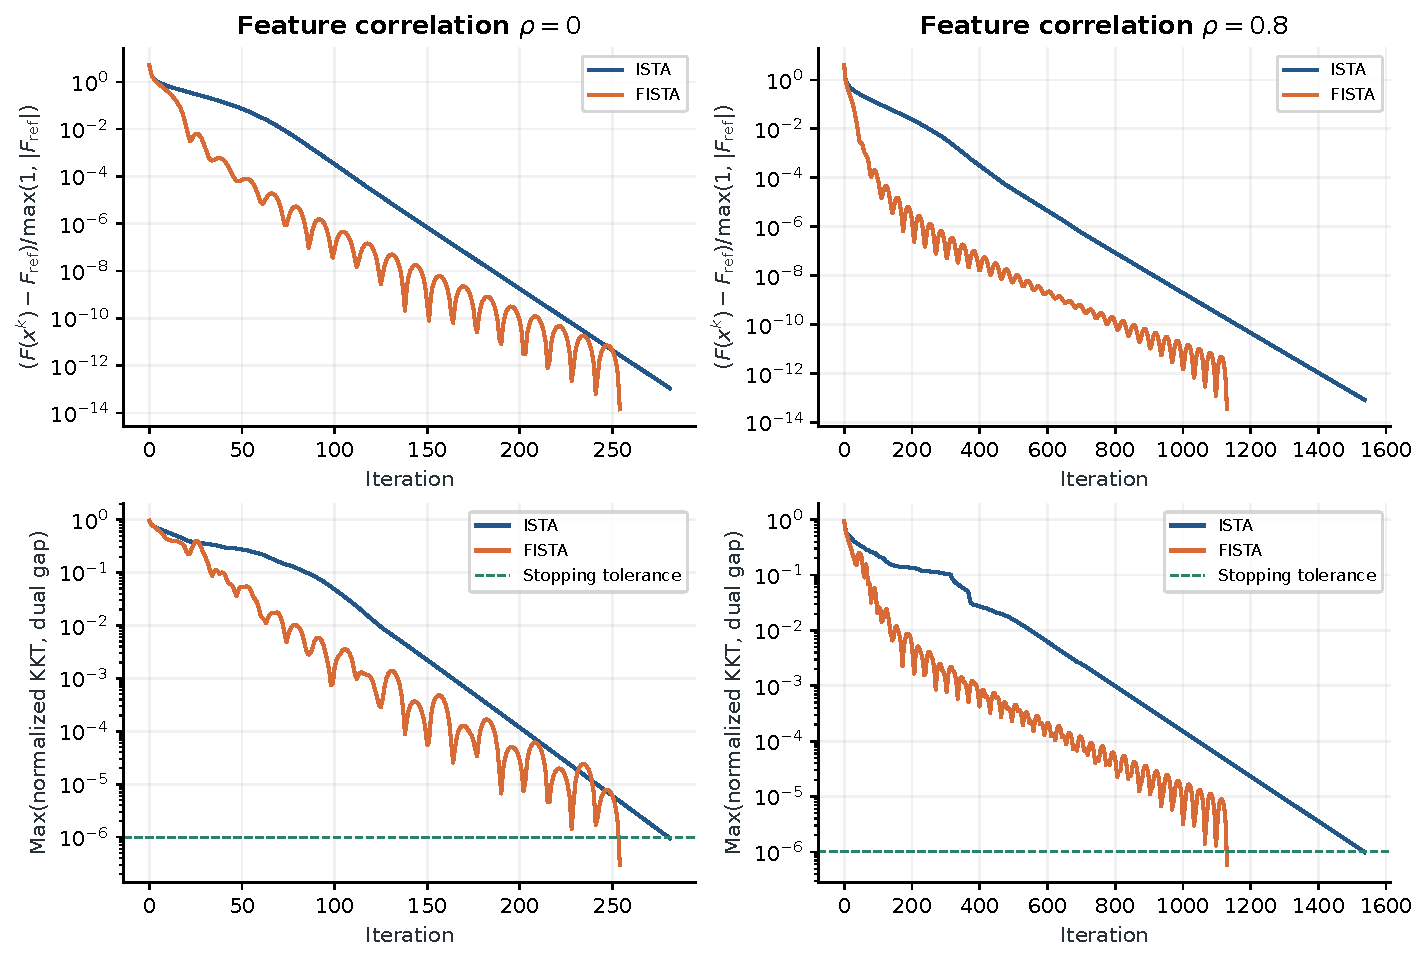
\includegraphics[width=\linewidth]{../figures/01_convergence.pdf}
\caption{种子 20261031 的收敛轨迹，上排为相对参照目标差，下排为共同停止指标。
目标差仅为对数作图在 $10^{-14}$ 处截断；真实终止依据为下排指标。FISTA 的非单调波动符合其标准形式的特点。}
\label{fig:convergence}\end{figure}

FISTA 在前期迅速降低目标值，但后期仍需要消除动量振荡并满足最优性条件。
因此图\ref{fig:convergence}中的早期优势与最终迭代数之比不必相同。
本实验没有通过拟合一段曲线去“证明”理论阶数，理论速率的依据是式\eqref{eq:istarate}和式\eqref{eq:fistarate}的上界。

\subsection{步长对 ISTA 的影响}
\begin{table}[htbp]
\centering\small
\caption{ISTA 步长实验（5 个种子）}\label{tab:steps}
\begin{tabular}{lrrr}
\toprule
步长 & 迭代次数 & 最大 $R_{\rm KKT}$ & 最大 $G_{\rm rel}$ \\
\midrule
$0.25/L$ & $1240.8\pm203.8$ & $9.54\times10^{-8}$ & $9.97\times10^{-7}$ \\
$0.5/L$ & $617.4\pm101.9$ & $9.49\times10^{-8}$ & $9.96\times10^{-7}$ \\
$1/L$ & $305.6\pm51.1$ & $9.37\times10^{-8}$ & $9.99\times10^{-7}$ \\
\bottomrule
\end{tabular}
\end{table}

在本组固定步长实验中，从 $0.25/L$ 增加到 $1/L$ 后，平均迭代次数由 \SmallStepIterations{}
降至 \FullStepIterations{}。较小步长虽然仍满足收敛条件，但每步移动有限，累计计算量更大。
这支持在已知可靠 $L$ 时使用 $1/L$；并不表示可以无限增大步长。
本文未测试超出保证范围的步长，也未比较回溯线搜索。

\begin{figure}[htbp]\centering
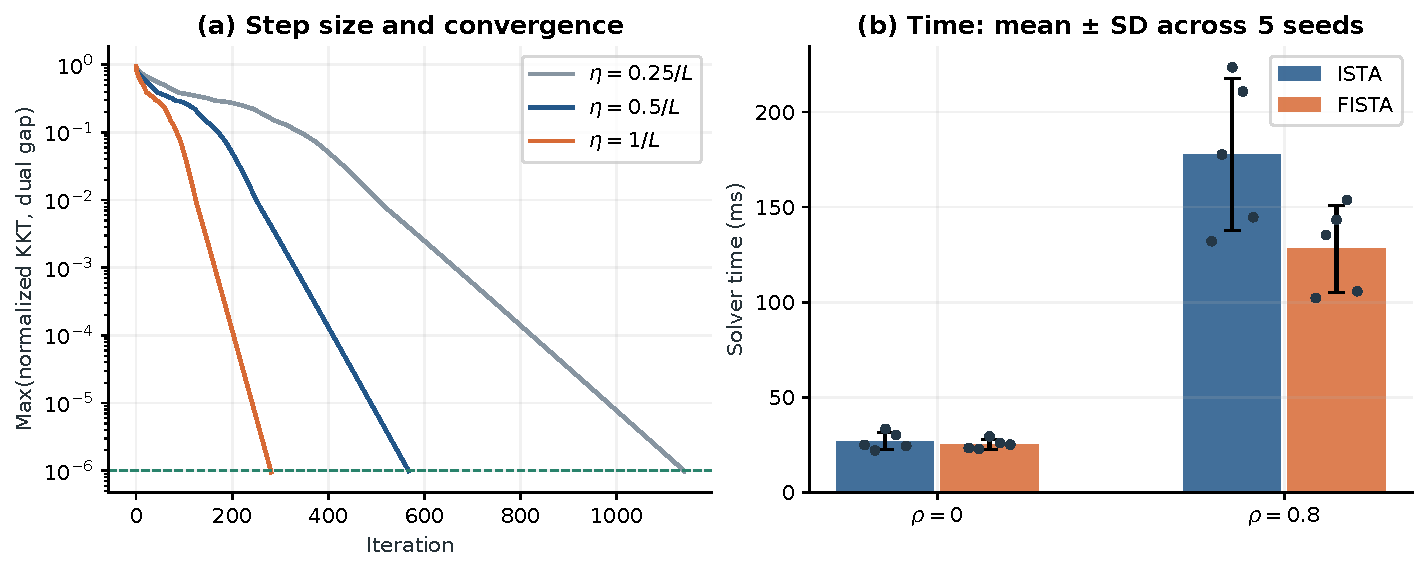
\includegraphics[width=\linewidth]{../figures/02_steps_and_time.pdf}
\caption{左：同一实例下 ISTA 的步长影响。右：算法时间均值与标准差；散点表示每个种子的三次计时中位数。}
\label{fig:steps}\end{figure}

\subsection{稀疏恢复与预测效果}
基础场景的 5 个种子均由验证集选出 $\lambda=0.03\lambda_{\max}$。
该组测试 MSE 为 \BaseMSE{}，参数相对误差为 \BaseError{}，
平均支持集精确率为 \BasePrecision{}、召回率为 \BaseRecall{}。
平均噪声方差为 \BaseNoiseVariance{}，逐种子计算的测试 MSE 与噪声方差之比平均为 \BaseNoiseRatio{}。
噪声方差是知道真实条件均值时的总体不可约预测误差，有限测试集 MSE 会在其附近波动。

\begin{table}[htbp]
\centering\small
\caption{基础场景下的统计模型比较（5 个种子）}\label{tab:baselines}
\begin{tabular}{lrrr}
\toprule
模型 & 测试 MSE & 参数相对误差 & 非零数 \\
\midrule
Lasso（验证集选参） & $0.348\pm0.057$ & $0.0738\pm0.0124$ & $77.0\pm20.7$ \\
最小范数最小二乘 & $16.212\pm1.286$ & $0.8449\pm0.0164$ & $1000.0\pm0.0$ \\
仅截距模型 & $22.662\pm1.332$ & $1.0000\pm0.0000$ & $0.0\pm0.0$ \\
\bottomrule
\end{tabular}
\end{table}


表\ref{tab:baselines}加入最小范数最小二乘和仅预测训练响应均值的模型作统计基线。
最小二乘通过 SVD 求最小范数解，且同样只使用训练数据；它不是另一种 Lasso 求解器。
本次稀疏高维设定下，Lasso 的测试误差低于这两项基线，体现了稀疏先验的作用。
此比较没有包含调参后的岭回归，因此不能扩展为“Lasso 优于所有正则化方法”。

\begin{figure}[htbp]\centering
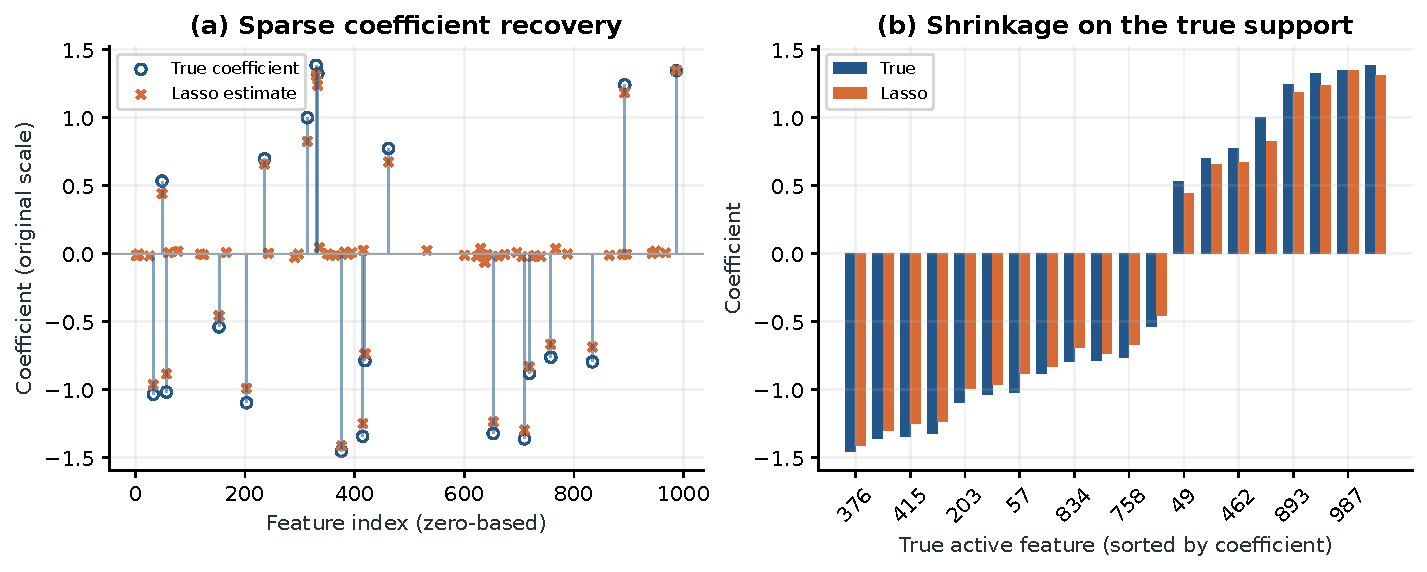
\includegraphics[width=\linewidth]{../figures/03_recovery.pdf}
\caption{基础场景、种子 20261031、验证集所选模型的参数恢复。
左图展示全部特征坐标中的真实和估计非零系数，右图按真实系数大小排列 20 个真实活跃变量。}
\label{fig:recovery}\end{figure}

在图\ref{fig:recovery}对应的单次实验中，模型选择 \ExampleNNZ{} 个变量，其中真阳性 \ExampleTP{} 个、假阳性 \ExampleFP{} 个。
模型能够识别真实活跃变量的主要幅度与符号，但还保留了小幅度的无关系数。
验证集 MSE 选择的目标是预测，而不是支持集完全恢复；较小的多余系数可能只带来有限的预测影响。
所以“检出了真实变量”与“只检出真实变量”必须分开判断，不能仅凭召回率高就认定精确恢复成功。

\FloatBarrier
\subsection{正则化参数的影响}
\begin{table}[htbp]
\centering\small
\caption{基础场景的正则化参数影响}\label{tab:regularization}
\begin{tabular}{lrrrrr}
\toprule
$\lambda/\lambda_{\max}$ & 测试 MSE & 参数误差 & 非零数 & 精确率 & 召回率 \\
\midrule
0.001 & $0.508\pm0.091$ & $0.1134\pm0.0108$ & $288.6\pm2.6$ & 0.069 & 1.000 \\
0.003 & $0.473\pm0.079$ & $0.1061\pm0.0096$ & $270.2\pm7.7$ & 0.074 & 1.000 \\
0.01 & $0.392\pm0.061$ & $0.0869\pm0.0091$ & $198.8\pm19.7$ & 0.101 & 1.000 \\
0.03 & $0.348\pm0.057$ & $0.0738\pm0.0124$ & $77.0\pm20.7$ & 0.274 & 1.000 \\
0.1 & $0.914\pm0.251$ & $0.1728\pm0.0308$ & $21.0\pm1.0$ & 0.954 & 1.000 \\
0.3 & $5.947\pm1.575$ & $0.5017\pm0.0677$ & $18.2\pm2.0$ & 1.000 & 0.910 \\
1 & $22.662\pm1.332$ & $1.0000\pm0.0000$ & $0.0\pm0.0$ & 0.000 & 0.000 \\
\bottomrule
\end{tabular}
\par\vspace{0.3em}{\footnotesize 前 3 项统计量为均值与样本标准差；精确率和召回率列仅列均值。}
\end{table}

\begin{figure}[htbp]\centering
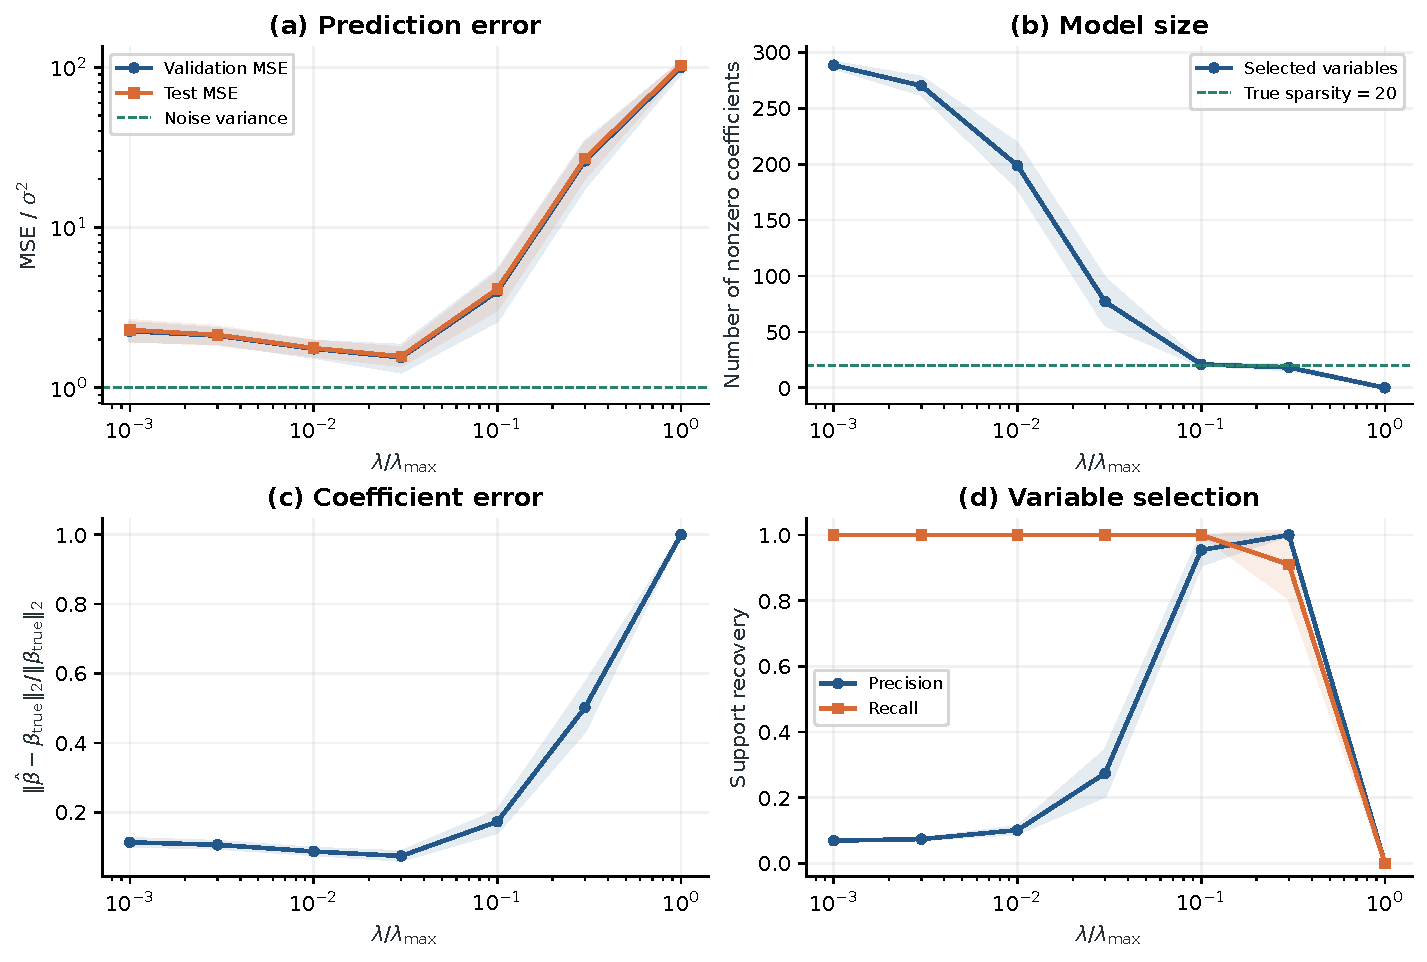
\includegraphics[width=\linewidth]{../figures/04_regularization.pdf}
\caption{基础场景的正则化实验；折线为 5 个种子均值，阴影为一个样本标准差。
测试误差曲线用于描述预先指定的参数网格，实际选参依据为各自验证集误差。}
\label{fig:regularization}\end{figure}

图\ref{fig:regularization}和表\ref{tab:regularization}展示三种区域。
正则化很弱时，模型保留较多变量，部分噪声也进入估计；适中惩罚在本实验中得到较低预测误差；
惩罚很强时，收缩偏差增大，真实变量可能被遗漏。
当比例达到 1，数值结果给出零系数模型，与式\eqref{eq:lambdamax}一致。
这里的零系数模型仍通过训练响应均值给出常数预测。
本次网格上模型大小总体随惩罚增大而减少，但一般 Lasso 路径中的单个变量可能进入后退出，
不能把有限网格结果理解为任意数据下支持集必然严格嵌套的定理。

\FloatBarrier
\subsection{样本量、噪声与特征相关性}
\begin{table}[htbp]
\centering\small
\caption{验证集选参后的单因素实验（每行 5 个种子）}\label{tab:sensitivity}
\begin{tabular}{lrrrr}
\toprule
场景 & 参数相对误差 & 测试 MSE & 非零数 & 支持集 F1 \\
\midrule
基础场景 & $0.0738\pm0.0124$ & $0.348\pm0.057$ & $77.0\pm20.7$ & $0.427\pm0.086$ \\
$n=150$ & $0.1291\pm0.0185$ & $0.602\pm0.126$ & $103.4\pm17.1$ & $0.329\pm0.045$ \\
$n=600$ & $0.0509\pm0.0062$ & $0.278\pm0.033$ & $73.8\pm70.9$ & $0.556\pm0.221$ \\
$\delta=0.05$ & $0.0368\pm0.0056$ & $0.087\pm0.014$ & $124.8\pm16.1$ & $0.279\pm0.032$ \\
$\delta=0.3$ & $0.2293\pm0.0392$ & $3.217\pm0.548$ & $88.0\pm58.0$ & $0.435\pm0.157$ \\
$\rho=0.5$ & $0.0775\pm0.0117$ & $0.349\pm0.064$ & $94.4\pm49.4$ & $0.390\pm0.119$ \\
$\rho=0.9$ & $0.1257\pm0.0168$ & $0.356\pm0.066$ & $117.8\pm16.1$ & $0.294\pm0.035$ \\
\bottomrule
\end{tabular}
\par\vspace{0.3em}{\footnotesize 基础场景为 $n=300,\ \rho=0,\ \delta=0.1$；每行只改变标出的一个因素。}
\end{table}

\begin{figure}[htbp]\centering
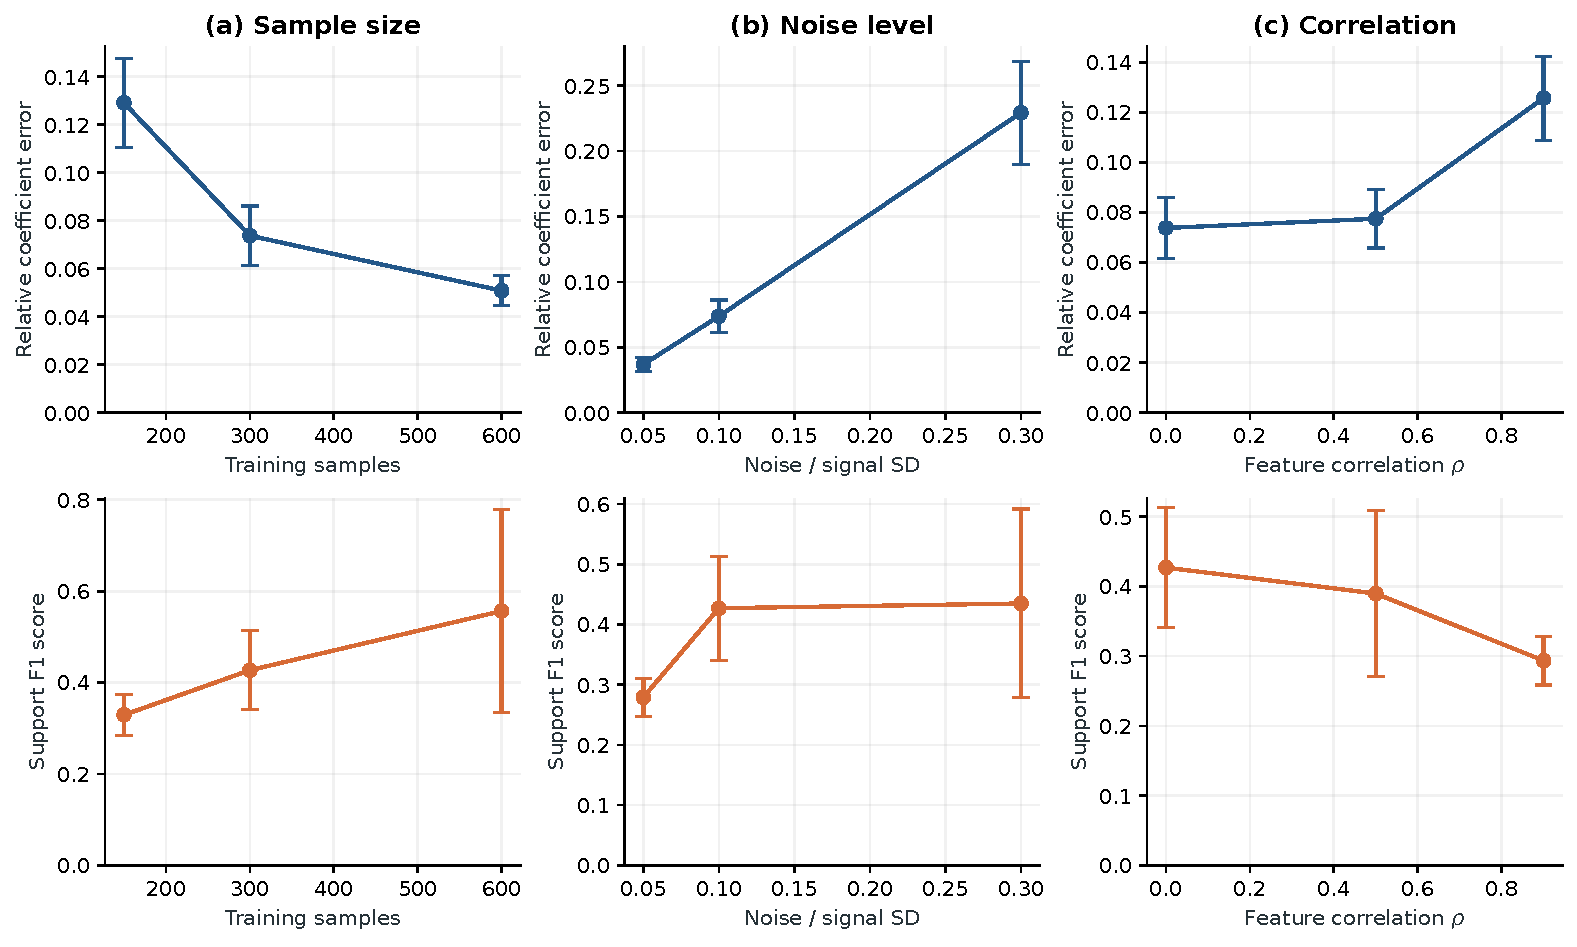
\includegraphics[width=\linewidth]{../figures/05_sensitivity.pdf}
\caption{三个单因素实验。每个数据集均由独立验证集从相同候选网格选参；误差棒为 5 个种子的样本标准差。
第一行衡量参数恢复，第二行衡量支持集恢复。}
\label{fig:sensitivity}\end{figure}

样本量从 150 增至 600 时，参数相对误差的均值从 \ErrorLowSample{} 降至 \ErrorHighSample{}，
测试 MSE 的均值从 \MSELowSample{} 降至 \MSEHighSample{}。
更多观测改善了本次问题中的参数辨识和泛化，但支持集 F1 仍受验证集选参目标影响，
不应预设其会随样本量严格单调变化。

噪声比例从 0.05 增至 0.3 时，参数相对误差均值从 \ErrorLowNoise{} 增至 \ErrorHighNoise{}。
不同噪声设定的绝对 MSE 同时包含不可约噪声的变化；因此还保存了以 $\sigma^2$ 归一化的预测指标，
避免将所有 MSE 增长都归因于求解算法。
低噪声组的参数误差更小，但其支持集 F1 反而低于基础场景。
这与验证集选出的更弱惩罚及更多小幅假阳性有关，不能解释为降低噪声本身不利于变量识别。

将相关系数从 0 增至 0.9 后，参数相对误差均值由 \BaseErrorMean{} 变为 \ErrorHighCorrelation{}。
强相关使若干特征具有相似解释能力，增加了准确区分系数与支持集的难度。
与此同时，两组平均测试 MSE 接近，体现了相关变量之间可能用不同系数组合产生相近预测。
表中反映的是“给定网格、验证集选择和稀疏信号分布”的联合结果，
不能把它全部归结为优化误差，因为这些求解均已经达到同一最优性准则。
仅有 5 个随机种子足以呈现实验现象，但不足以据此作广泛的统计显著性声明。
\FloatBarrier

\section{结论与局限}
本研究完成了 Lasso 的建模、近端更新推导、ISTA/FISTA 独立实现与实际数值验证。
核心结果可以归纳为以下几点：
\begin{enumerate}
\item $\ell_1$ 正则项的近端算子具有软阈值闭式解，使每轮迭代仅需矩阵--向量乘法和逐坐标阈值运算。
固定步长 $1/L$ 下，ISTA 在本研究中稳定达到统一精度；与独立坐标下降解的目标值相符。
\item FISTA 在本次两组算法基准中减少了平均迭代数；具体时间收益受数据相关性、动量振荡、证书精度和实现开销影响。
理论的 $O(1/k^2)$ 目标误差界不等于逐步单调下降，也不等于任意停止准则下的固定倍数加速。
\item 正则化控制预测与稀疏性的权衡。验证集选出的模型能够较好预测，却仍存在假阳性变量；
优化精确、预测良好、支持集精确恢复是三个不同层次的结论。
\item 增加样本量在本次设定下改善了参数恢复，而高噪声和强相关增加了恢复难度。
采用训练集预处理、独立验证集选参和独立测试评价，能避免将信息泄漏误认为模型性能提升。
\end{enumerate}

本文的局限包括：使用合成线性高斯数据，不能直接证明对真实业务场景的适用性；
候选 $\lambda$ 网格较粗，且采用一次验证划分；仅进行 5 次随机重复；未研究稀疏矩阵、大规模分布式计算、
自适应重启、回溯步长或非高斯噪声。后续可加入真实数据、交叉验证及更密的参数网格，
并根据实际任务分别设计预测评价与变量筛选评价。

\appendix
\section{代码公开与复现说明}
本文的算法实现、实验配置、原始结果、图表及报告源文件已公开于
\url{https://github.com/10255102560/Lasson}，可供核验与复现。
实验结果对应的初始公开版本为
\href{https://github.com/10255102560/Lasson/commit/eeaed69b0accff24bd4aac847baed2e1798f91ef}{\texttt{eeaed69}}；
运行环境与源文件校验信息见 \texttt{results/metadata.json}。

\begin{table}[htbp]\centering\small
\caption{主要配套文件}
\begin{tabular}{p{5cm}p{7.9cm}}
\toprule 文件 & 内容\\\midrule
\texttt{lasso.py} & 软阈值、谱常数、ISTA/FISTA 和最优性证书。\\
\texttt{data.py} & 随机问题生成、训练集预处理和统计指标。\\
\texttt{experiment\_config.json} & 预先固定的随机种子、网格和实验场景。\\
\texttt{run\_experiments.py} & 完整实验、计时及 CSV/NPZ 记录。\\
\texttt{make\_figures.py} & 从原始结果生成 5 组图表和汇总 CSV。\\
\texttt{verify\_results.py} & 核验结果完整性、最优性、选参和源文件哈希。\\
\texttt{build\_report.py} & 从结果生成数值表、PDF 及可编辑 Word 报告。\\
\texttt{tests/test\_lasso.py} & 6 项数学与实现正确性检查。\\
\texttt{results/} & 原始指标、迭代轨迹、参考检查、环境版本和基础问题快照。\\
\texttt{figures/} & 适合排版的 PDF 矢量图及 PNG 图片。\\
\texttt{report/lasso\_report.tex} & 本报告的 LaTeX 源文件。\\
\bottomrule\end{tabular}\end{table}

可使用以下命令获取仓库。在安装好 Python 依赖后，于项目根目录运行后续命令：
\begin{verbatim}
git clone https://github.com/10255102560/Lasson.git
cd Lasson
python -m unittest discover -s tests -v
python run_experiments.py
python verify_results.py
python make_figures.py
python build_report.py
\end{verbatim}
完整实验本次实际耗时约 \TotalSeconds{} 秒，不包含环境安装、绘图和文档编译；不同硬件耗时会变化。
PDF 重新编译需要含 CTeX 的 XeLaTeX 环境；Word 导出需要配套的 Pandoc 依赖。
若仅需复核结果，可以直接读取 \texttt{results/} 下的 CSV，无须重新运行实验。
模型数值由固定种子和版本信息复现，运行时间不会逐位相同。
详细环境安装、Apple Silicon 后端说明和文件使用方式见根目录的 \texttt{README.txt}。

\begin{thebibliography}{9}
\small\setlength{\itemsep}{0pt}\setlength{\parskip}{0pt}
\bibitem{tibshirani} Tibshirani R. Regression Shrinkage and Selection via the Lasso.
Journal of the Royal Statistical Society: Series B, 1996, 58(1): 267--288.
\href{https://doi.org/10.1111/j.2517-6161.1996.tb02080.x}{doi:10.1111/j.2517-6161.1996.tb02080.x}.
\bibitem{daubechies} Daubechies I, Defrise M, De Mol C.
An iterative thresholding algorithm for linear inverse problems with a sparsity constraint.
arXiv:math/0307152, 2003.
\url{https://arxiv.org/abs/math/0307152}.
\bibitem{beck} Beck A, Teboulle M. A Fast Iterative Shrinkage-Thresholding Algorithm for Linear Inverse Problems.
SIAM Journal on Imaging Sciences, 2009, 2(1): 183--202.
\href{https://doi.org/10.1137/080716542}{doi:10.1137/080716542}.
\bibitem{sklearn} scikit-learn developers. Lasso: scikit-learn 1.6.1 documentation.
\url{https://scikit-learn.org/1.6/modules/generated/sklearn.linear_model.Lasso.html}.
访问日期：2026-10-31。
\end{thebibliography}
\end{document}
